\chapter{Fundamentals}

\section{Differential Privacy}

Differential Privacy ist ein Verfahren, dass die Privatheit bei interaktiven Anfragen auf Datenbanken schützen kann. Es wurde in \cite{dwork:2006} formalisiert, nachdem gezeigt wurde, dass Anforderungen an Privatheit aus \cite{dalenius:1977} in der Praxis nicht umsetzbar sind. In \cite{dalenius:1977} war die Philosophie, dass ein Angreifer nichts lernen soll, was er nicht auch ohne Zugriff auf die Datenbank hätte lernen können. \textcite{dwork:2006} zeigt, dass diese Definition aufgrund von Hilfsinformationen, die der Angreifer besitzen kann nicht umsetzbar ist. Stattdessen verfolgt \textcite{dwork:2006} mit der Differential Privacy einen Ansatz, bei dem nicht direkt das Wissen des Angreifers einbezogen wird, sondern ob der Angreifer bei einer bestimmten Anfrage mehr über ein Individuum lernen kann, wenn es in der zugrundeliegenden Datenbank ist.

Formal vergleicht Differential Privacy die Wahrscheinlichkeit ein ähnliches Anfrageergebnis zu erhalten, wenn ein Individuum in einer Datenbank ist oder nicht. Je weniger diese Wahrscheinlichkeiten auseinander liegen, desto weniger kann ein Angreifer durch die Präsenz des Individuums in der Datenbank lernen und desto höher ist die Privacy. Die Definition aus \cite{dwork:2006} ist folgende:

\begin{definition}\label{def:eps-differential-privacy}
	\emph{\textbf{$\epsilon$-Differential Privacy}} A \textit{randomized mechanism} $\mathcal{M}: \mathcal{D} \rightarrow \mathcal{R}$ with domain $\mathcal{D}$ and range $\mathcal{R}$ satisfies $\epsilon$-differential privacy if for any two adjacent inputs $d$, $d' \in \mathcal{D}$ and for any subset of outputs $S \subseteq \mathcal{R}$ it holds that $$\Pr[\mathcal{M}(d) \in S] \leq e^{\epsilon} \Pr[\mathcal{M}(d') \in S]$$
\end{definition}

Hervorzuheben ist hierbei noch, dass die Definition keine Anforderungen an die Datenbanken $d, d'$ macht, außer, dass sie benachbart sind. Typischerweise gilt dafür die folgende Definition:
% Quelle hinzufügen? Bzw. klar machen warum ich sie hier explizit aufschreibe, nämlich in abgrenzung zu den User-adjacent datasets\cite{mcmahan:2018}
\begin{definition}\label{def:example-adjacency}
	\emph{\textbf{Example-adjacent datasets}} Two datasets $d$ and $d'$ are defined to be example-adjacent if $d'$ can be formed by adding or removing a single example from $d$.
\end{definition}

Wenn in dieser Arbeit von benachbarten Datensätzen die Rede ist, gilt i.A. diese Definition, wenn nicht explizit anders beschrieben.

Eine leicht abgeschwächte Version der Definition fügt einen Parameter $\delta$ hinzu, der die Wahrscheinlichkeit repräsentiert, dass die Privatheitsgarantien nicht eingehalten werden. Er sollte demenstprechend sehr klein gewählt werden.\cite{dwork:2014} 

\begin{definition}\label{def:eps-delta-differential-privacy}
	\emph{\textbf{$(\epsilon, \delta)$-Differential Privacy}} A \textit{randomized mechanism} $\mathcal{M}: \mathcal{D} \rightarrow \mathcal{R}$ with domain $\mathcal{D}$ and range $\mathcal{R}$ satisfies $(\epsilon, \delta)$-differential privacy if for any two adjacent inputs $d$, $d' \in \mathcal{D}$ and for any subset of outputs $S \subseteq \mathcal{R}$ it holds that $$\Pr[\mathcal{M}(d) \in S] \leq e^{\epsilon} \Pr[\mathcal{M}(d') \in S] + \delta$$
\end{definition}

Um die Definitionen zu erfüllen wird auf ein Anfrageergebnis von $\mathcal{M}$ Rauschen hinzugefügt. Die Varianz der Verteilung, aus der das Rauschen gezogen wird hängt von der Sensitivität einer Anfrage ab. Sie beschreibt die größtmögliche Veränderung für eine Anfrage, die durch das Hinzufügen oder das Löschen eines Eintrags auftreten kann.\cite{dwork:2006}

\begin{definition}\label{def:l1-sensitivity}
	\emph{\textbf{L1-Sensitivity}} For $\mathcal{M}: \mathcal{D} \rightarrow \mathcal{R}^{d}$, the L1-Sensitivity of $\mathcal{M}$ is 
	$$
	\Delta \mathcal{M} = \max_{d_1, d_2}{||\mathcal{M}(d_1) - \mathcal{M}(d_2)||}_1
	$$
	for all adjacent datasets $d_1$, $d_2$
\end{definition}

Das Rauschen wird je nach Anwendungsfall aus verschiedenen Verteilungen gezogen. Beispielsweise gibt es den Laplace- oder den Gauss'schen Mechanismus, um numerische Anfragen, beispielsweise Durchschnitt einer Datenbank, privat zu machen. Für Anfragen, die ein Ergebnis aus einer festgelegten Menge liefern sollen, gibt es den Exponentiellen Mechanismus. Dieser bewertet die potenziellen Ergebnisse anhand einer Bewertungsfunktion.\cite{mcsherry:2007}

Bei den Mechanismen ist variiert die Definition der Sensitivität leicht, beispielsweise nutzt der Gauss'sche Mechanismus die $\ell_2$-Norm anstatt der $\ell_1$-Norm, die Intuition, dass es um die maximale Abweichung im Anfrageergebnis durch ein Individuum geht, bleibt jedoch immer erhalten. Darüber hinaus erfüllt der Laplace Mechanismus $\epsilon$-Differential Privacy, der Gauss'sche Mechanismus jedoch nur $(\epsilon, \delta)$-Differential Privacy.\cite[p.261ff]{dwork:2014}

Mit den bisher erwähnten Methoden kann die Privatheit einzelner Anfragen gewährleistet werden. Wenn die gleichen Anfragen aber zum Beispiel mehrfach gestellt werden muss auch das Niveau der Privatheit abnehmen, da der Durchschnitt der einzelnen Anfragen irgendwann gegen den echten Wert konvergiert.\cite[p.42]{dwork:2014} Ein großer Vorteil von Differential Privacy ist, dass sich diese Verringerung der Privatheit abschätzen lässt. Dafür gibt es einige Kompositionstheoreme:

% Kompositionstheoreme einfügen
\begin{itemize}
	\item Group Privacy
	\item Sequential Composition
	\item Parallel Composition
	\item Complex Composition Theorem(?)
	\item Strong Composition Theorem(?)\cite{dwork:2010}
\end{itemize}

Darüber hinaus können Ergebnisse, die durch einen Mechanismus erhalten wurden der Differential Privacy erfüllt, weiterverarbeitet werden, ohne dass die Privatheit weiter kompromittiert wird (\textit{post-processing}).\cite{dwork:2014}

\subsection{Differential Privacy in Machine Learning}
Es gibt verschiedene Punkte, an denen Differential Privacy im Machine Learning ansetzen kann um die Privatheit zu gewährleisten. Jeder Punkt hat verschiedene Vor- und Nachteile, die ich im Folgenden umreiße. Eine Übersicht dazu ist in \autoref{fig:design_principles_dpml} zu sehen.

\begin{figure}[tb]
	\centering
	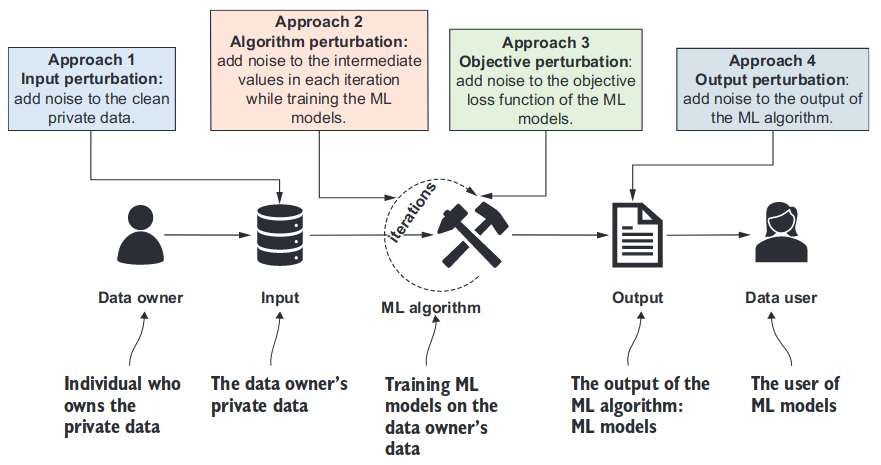
\includegraphics[width=0.7\textwidth]{Bilder/design_principles_dpml.png}
	\caption{Design principles of differentially private ML from \textcite{chang:2023}}
	\label{fig:design_principles_dpml}
\end{figure}

Bei der \textit{Input Pertubation} wird den Trainingsdaten Rauschen hinzugefügt, bevor das Modell mit ihnen trainiert wird. Dieser Ansatz ist ohne weitere Änderungen am Trainingsalgorithmus oder am Modell anwendbar, da der Trainingsalgorithmus dann Daten verarbeitet, die bereits differential private sind und es damit einem \textit{post-processing} entspricht. Das Modell kann danach also problemlos weiterverwendet werden. Ein großer Nachteil ist aber, dass die Anfragen auf den Trainingsdaten im Allgemeinen eine hohe Sensitivität haben und daher viel Rauschen hinzugefügt werden muss.

Die \textit{Algorithm Pertubation} ist das am weitesten verbreitete Verfahren und liegt großen Bibliotheken wie Opacus\cite{yousefpour:2021} und TensorFlow Privacy\cite{tfprivacy} zugrunde. Es kann für iterative Optimierungsverfahren wie Gradient Descent oder die Power Iteration Methode bei einer Principal Component Analysis (PCA) genutzt werden. 

Bei der Anwendung dieses Verfahrens im Gradient Descent wird Differential Privacy auf die Updates der Gradienten angewendet, das heißt diese werden für gewöhnlich auf eine bestimmte Vektornorm gestutzt und dann wird basierend darauf Rauschen addiert. In der Regel muss hierbei deutlich weniger Rauschen hinzugefügt werden, als bei der \textit{Input Pertubation}.\cite{chang:2023} Der \textit{Privacy Loss}, der durch einen Trainingsdurchlauf anfällt, kann mithilfe von Kompositionstheoremen bestimmt werden. Für die Abschätzung wurde das \textit{Strong Composition Theorem}\cite{dwork:2010} genutzt, allerdings konnten \textcite{abadi:2016} mit dem \textit{Moments Accountant} eine deutlich genauere Abschätzung für das Training von Neuronalen Netzen liefern. So können Neuronale Netze mit dem Verfahren bereits mit kleinen Privacy Budgets trainiert werden. Das trainierte Modell kann ebenfalls veröffentlicht werden, da dessen Gewichte die Anforderungen der Differential Privacy erfüllen.

\textit{Objective Pertubation} verändert die Zielfunktion des Trainings. Statt auf die Daten wird während des Trainings Rauschen auf diese Funktion gelegt.

Bei der \textit{Output Pertubation} wird ein nicht-privates Modell trainiert und nur die Ausgabe des Modells verrauscht. Dieses Verfahren hat den großen Nachteil, dass es nicht anwendbar ist, wenn das Modell veröffentlicht werden soll.

% Verfahren nutzt auch den Moments Accountant
% Teacher müssen privat trainiert werden (?)
% bei Teachern wird Output Pertubation angewendet
Ein Vertreter dieses Ansatzes ist \textit{PATE}\cite{papernot:2017}. Hierbei werden \textit{Teacher Models} auf disjunkten Teilmengen der sensitiven Trainingsdaten trainiert. Das Ensemble dieser \textit{Teacher Models} trainiert danach ein \textit{Student Model} auf einem nicht-sensitiven oder öffentlichen Datensatz. Diese Daten müssen nicht gelabelt sein, da die trainierten \textit{Teacher Modelle} die Labels generieren. Vorteil dieses Verfahrens ist, dass es keine Anforderungen an die Modelle oder den Trainingsprozess stellt. Auch die \textit{Teacher Models} können nicht privat trainiert werden. Die Privatheit entsteht dadurch, dass auf die Ausgabe des Ensembles mit dem \textit{Laplace Mechanismus} Rauschen hinzugefügt wird. Das entspricht der \textit{Output Pertubation}. Da die wiederholte Anfrage der \textit{Teacher Modelle} den Verlust an Privacy erhöht, wird nur eine vorher festgelegte Anzahl an ungelabelten Daten für das \textit{Student Model} mit Labels versehen. Dabei wird nur das mit der größten Konfidenz vorhergesagte Label genutzt. So lässt sich der \textit{Privacy Loss} mithilfe von Kompositionstheoremen abschätzen. Das so trainierte \textit{Student Model} hat diese Limitierung nicht und kann veröffentlicht werden.

Abgesehen von der Varianz des Laplaceschen Rauschens ist die Anzahl der \textit{Teacher Models} wichtig für den Trade-Off zwischen Privacy und Genauigkeit. Eine größere Anzahl an \textit{Teacher Models} verringert den Verlust an Privacy, allerdings wird auch deren Genauigkeit verhindert, da die Menge der Trainingsdaten pro \textit{Teacher Model} abnimmt.

\textcite{papernot:2017} evaluieren \textit{PATE} auf MNIST und SVHN. Im Fall von SVHN nutzen sie die \textit{Extended Version} des Datensatzes und betonen, dass die größere verfügbare Menge an Trainingsdaten die zusätzliche Komplexität des Datensatzes kompensiert. Mit 250 \textit{Teacher Models} können sie Genauigkeiten von $98\%$ (MNIST) und $90.66\%$ (SVHN) erzielen. Das Ergebnis auf MNIST kann damit \textcite{abadi:2016} schlagen.

Der größte Nachteil an PATE ist, dass der Algorithmus nicht-private (potenziell ungelabelte) Daten benötigt, da das \textit{Student Model} nicht-privat trainiert wird. Diese Voraussetzung braucht der Algorithmus von \textcite{abadi:2016} nicht.

\subsection{Individualized Differential Privacy}

Motiviert von den verschiedenen Anforderungen und Präferenzen unterschiedlicher Personen an die Privatheit ihrer Daten haben \textcite{alaggan:2016} und wenig später unabhängig \textcite{jorgensen:2015} Arbeiten zu Differential Privacy mit individuellen Privacy Budgets veröffentlicht.

% muss überarbeitet / überprüft werden, kurz vor Schluss geschrieben
\textcite{alaggan:2016} definieren heterogene Differential Privacy im Kontext von Nutzerprofilen. In ihrer Arbeit individualisieren sie die Privacy durch das Anpassen der Sensitivität der Komponenten mit unterschiedlichen Budgets. Dazu erstellen sie eine \textit{Shrinkage Matrix}, mit der die Datenpunkte multipliziert werden. Die Matrix ist eine Diagonalmatrix, bei der die Diagonalelemente in $[0;1]$ liegen und abhängig von dem jeweiligen Privacy-Budget sind.

Ihr Ansatz ist jedoch für einige Funktionen nicht anwendbar, beispielsweise können das Minimum und die $\ell_0$-Norm nicht berechnet werden.

\textcite{jorgensen:2015} stellen einen Sampling Ansatz vor, mit dem beliebige DP-Algorithmen in einen Algorithmus mit individualisierter DP überführt werden können. Dabei wird der zugrundeliegende DP-Algorithmus als Black Box betrachtet und die Wahrscheinlichkeit, dass ein Tupel für den Algorithmus gezogen wird, davon abhängig gemacht, was der Nutzer als Privacy Budget gewählt hat.

In ihren Experimenten betrachten sie das gewählte Privacy Budget eines Nutzers als öffentliche Information. Dies kann als problematisch gewertet werden, da es theoretisch etwas über die Wichtigkeit einer Information aussagen kann. Sie rechtfertigen diesen Umstand damit, dass die Budgets nicht für ein Attribut gewählt werden sondern für ein Individuum mit potenziell vielen Attributen und diese Information daher nur etwas über die Person aussagt. Darüber hinaus plädieren sie dafür, einen Nutzer anstatt eines genauen Budgets eine bestimmte Privatheitsstufe mit angemessener Beschreibung (niedrig, mittel und hoch) zu spezifizieren.

Darüber hinaus zeigen sie ein weiteres Verfahren basierend auf dem \textit{Exponential Mechanism}. Diesen verändern sie dazu so, dass die Score-Funktion die individuellen Privacy Budgets mitbetrachtet. Sie wenden diesen Mechanismus auf \textit{Count}, \textit{Median} und \textit{Min} an, merken aber an, dass das Finden eines Algorithmus, der die angepasste Score-Funktion für beliebige Funktionen effizient berechnet, nicht trivial ist.

Sie weisen die Effektivität ihrer Verfahren in Experimenten nach, in denen sie beide Verfahren für \textit{Count} und \textit{Median} durchführen und eine \textit{Multiple Linear Regression} mit dem Sampling-Verfahren. Ihre Verfahren vergleichen sie mit Standard-DP Verfahren und bei \textit{Count} zusätzlich mit den Stretching-Verfahren aus \cite{alaggan:2016}. Die Privacy Budgets teilen sie in drei Gruppen mit aufsteigenden Privacy-Budgets auf (\textit{conservative}, \textit{moderate} und \textit{liberal}). Bei \textit{Count} leidet das Sampling-Verfahren dadurch, dass Elemente augeschlossen werden. Allerdings kann der angepasste \textit{Exponential Mechanism} gute Ergebnisse liefern und das Stretching-Verfahren deutlich schlagen. \textit{Median} ist verhält sich gegenüber dem Sampling deutlich resistenter, weshalb der Ansatz hier auch gute Ergebnisse erzielen kann und auch besser abschneidet als der modifizierte \textit{Exponential Mechanism}. 

Auch bei der linearen Regression kann der Sampling Ansatz das Verfahren von \cite{alaggan:2016} schlagen. Der modifizierte \textit{Exponential Mechanism} ist hier nicht anwendbar.

\section{Federated Learning}

Federated Learning (FL) ist ein Optimierungsverfahren, bei dem einzelne Clients gemeinsam über mehrere Runden ein Modell trainieren, ohne dabei ihre eigenen Trainingsdaten mit anderen zu teilen. 

Das Verfahren umfasst einen Server, der den Ablauf des Trainings steuert und eine beliebige Anzahl von Clients, die das lokale Training auf ihren eigenen Daten durchführen. Der generelle Ablauf einer Trainingsrunde sieht wie folgt aus: 

\begin{enumerate}
	\item der Server initialisiert ein Modell und dessen Parameter (nur erste Runde) 
	\item \label{round-start} er eine Menge an Clients aus, mit denen in dieser Runde das Modell trainiert werden soll
	\item das Modell wird an die ausgewählten Clients geschickt
	\item die Clients optimieren das Modell auf ihren eigenen Daten und schicken die aktualisierten Parameter zurück an den Server
	\item der Server aggregiert die Parameter der Clients und konstruiert daraus neue Modellparameter; danach geht es in der nächsten Runde mit \autoref{round-start} weiter
\end{enumerate}

Die lokale Optimierung und die Aggregation der Updates variiert je nach Algorithmus. Die beiden Standardalgorithmen sind \texttt{FedAvg} und \texttt{FedSGD}\cite{mcmahan:2016}. Der wichtigste Unterschied ist, dass \texttt{FedAVG} die Clients mehrere Epochen auf ihren eigenen Daten trainieren lässt, während die Clients im \texttt{FedSGD} nur einen Schritt machen, bevor sie ihre aktualisierten Parameter wieder an den Server schicken. In beiden Algorithmen werden die Updates bei der Aggregation nach der Menge an Datenpunkten beim jeweiligen Client gewichtet.

Das verteilte Training kann vor allem zwei Probleme mit sich bringen. Zunächst kann der Overhead für die Kommunikation sehr groß werden, gerade wenn über viele Runden hinweg trainiert wird. Zum anderen kann nicht angenommen werden, dass die Daten über die Clients hinweg IID sind, was die Konvergenz der Algorithmen beeinträchtigen kann. \textcite{karimireddy:2020} versuchen diesem Problem zu begegnen, indem sie in ihrem Algorithmus die generelle Richtung, in die die Clients optimieren, an die Clients schicken und diese sie in ihre Updates einfließen lassen.

Die Anwendungsfälle von Federated Learning können variieren: Zum einen gibt es das \textit{Cross-device Federated Learning} und zum anderen das \textit{Cross-silo Federated Learning}\cite{kairouz:2021}. 

Ersteres entspricht dem Fall, dass die Clients eine Vielzahl von mobilen oder IoT-Geräten sind. Hierbei sind die Clients sehr unzuverlässig, zum Beispiel kann der Empfang zu schlecht werden, die Geräte ausgeschaltet werden oder wegen einem zu niedrigen Akkustand ungeeignet für die Teilnahme am Training sein. All dies kann von dem Server nicht beeinflusst werden, also muss das Trainingsverfahren mit solchen Ausfällen zurecht kommen. Darüber hinaus kann die Menge der Clients von dem Server nicht indiziert werden, da Geräte auch dauerhaft ausfallen können, zum Beispiel wenn ein Mobiltelefon kaputt geht oder ein neues gekauft wird und deshalb laufend neue Geräte hinzukommen können.

Bei dem \textit{Cross-silo Federated Learning} geht es vor allem um das Trainieren von Modellen zwischen unterschiedlichen Datencentern oder Organisationen. Die Motivation hierbei ist vor allem, dass es ein gemeinsames Interesse mehrerer Parteien an aussagekräftigen Modellen gibt, die zugrundeliegenden Trainingsdaten aber nicht den anderen Organisationen bereitgestellt werden sollen. Hierbei ist die Ausfallsicherheit der Clients deutlich höher als beim \textit{Cross-device Federated Learning} und auch die Menge der Clients ist in der Regel bekannt.

Auch der Server selbst kann bei einer sehr großen Zahl an Clients zu einem Bottleneck werden.\cite[p.11]{kairouz:2021} Daher wird ebenfalls an vollständig verteilten Trainingsverfahren geforscht, bei denen kein zentraler Server nötig ist (\textit{Fully-decentralized learning}).

\subsection{Data heterogeneity}

Ein generelles Problem beim Federated Learning ist die Heterogenität der Trainingsdaten. Da die Daten von unterschiedlichen Parteien generiert werden ist eine zufällige Verteilung der abhängigen und unabhängigen Variablen in der Regel nicht gegeben. Diese Heterogenität kann sich auf verschiedene Arten ausdrücken, wie im folgenden beschrieben.

\subsubsection{Intra-Client Distribution Skew}
Die Daten der einzelnen Clients können Abhängigkeiten aufweisen, beispielsweise wenn sie in einer zeitlichen Abfolge sortiert vorliegen. Derartige Abhängigkeiten können aber durch das Durchmischen der einzelnen Datenpunkte gelöst werden.

\subsubsection{Feature Distribution Skew}
Die Verteilung der Features kann sich zwischen den Clients unterscheiden, auch wenn die Wahrscheinlichkeit der Labels gegeben der Features, $P(y|x)$, die gleiche ist. Beispielsweise könnte es sein, dass eine Person sehr viele Hundebilder auf ihrem Handy hat, weil sie ein Hund als Haustier hat und eine andere Person sehr viele Katzenbilder, weil sie mit einer Katze wohnt.

\subsubsection{Label Distribution Skew}
Die Verteilung der Labels auf den Clients kann sich unterscheiden, zum Beispiel aufgrund von regionalen Unterschieden. Beispielsweise können Kängurus fast nur in Australien beobachtet werden.

\subsubsection{Other Distribution Skews}
Darüber hinaus werden weitere Verzerrungen erwähnt. Es kann sein, dass die bedingten Wahrscheinlichkeiten von Features und Labels sich unterscheiden, beispielsweise sieht ein Haus in den USA anders aus als in Europa, in beiden Fällen ist es aber ein Haus (\textit{concept drift}). Andersherum kann es auch sein, dass die gleichen Features anders gelabelt sind, beispielsweise weil manche Daten auch für Menschen ununterscheidbar sind.

\subsection{Privacy model in Federated Learning}
% local vs global (trusted server), record vs user level
Die bisherige Definition von Differential Privacy geht davon aus, dass die Privatheit einzelner Datenpunkte in einer Datenbank geschützt wird. Im Federated Learning ist die Struktur der Daten eine andere: Es gibt viele Clients und es ist wichtig die Privatheit des ganzen Datensatzes eines Clients zu schützen. Es reicht nicht aus einzelne Zeilen seiner Daten zu schützen. Wenn die Menge der Daten aller Clients als Datenbank angesehen wird, kann die Definition der benachbarten Datensätze aus  \autoref{def:example-adjacency} dementsprechend angepasst werden:

\begin{definition}\label{def:user-adjacency}
	\emph{\textbf{User-adjacent datasets}\cite{mcmahan:2018}} Let $d$ and $d'$ be two datasets of training examples, where each example is associated with a user. Then, $d$ and $d'$ are \textbf{adjacent} if $d'$ can be formed by adding or removing all of the examples associated with a single user from d.
\end{definition}

Mit dieser Definition kann gewährleistet werden, dass die Anwesenheit oder Abwesenheit der Trainingsdaten eines Nutzers nur einen unmerklichen Einfluss auf die Modellparameter des am Ende vom Lernprozess veröffentlichten Modells hat \cite{mcmahan:2018}.

Darüber hinaus kann Differential Privacy auf zwei Arten angewendet werden: lokal oder global. Bei der globalen Anwendung erfüllt wie oben beschrieben das Modell am Ende Differential Privacy. Allerdings sind die Parameterupdates, die an den Server geschickt werden nicht privat, denn das nötige Rauschen wird nur auf das Modellupdate angewendet, dass aus den Updates aller Clients aggregiert wird. Es muss also dem Server vertraut werden \cite[p.44]{kairouz:2021}.

Alternativ dazu ist die lokale Anwendung von Differential Privacy. Dabei muss das Rauschen hinzugefügt werden, bevor der Client sein Update an den Server schickt. In der Praxis hat sich allerdings gezeigt, dass dieser Ansatz schwierig umzusetzen ist\cite[p.54]{kairouz:2021}.